\chapter{Implémentation et Validation}
\label{ch:implem}

\subsection{Implémentation : EA dirigée par les modèles exécutables}
Implémentation du métamodèle avec Ecore avec EMF et co

Vue intégration : Contrainte OCLinEcore
Simulation 
Plugin fUML pour l'exécution de processus métier et la simulation de processus - fUML pour les Smart Grids et pour l'outil papyrus qui permet d'appeler des applications extérieures
Requête OCLinEcore pour mener l'analyse du comportement
Transformation de modèles 

\subsection{Validation application au cas d'étude}

Nous éprouvons notre démarche au cas métier de la gestion d'une flotte de véhicules électriques. Nous construisons les modèles adéquats pour les vues métier, fonctionnelle et applicative en adoptant des langages exécutables. La cohérence est modélisée dans la vue intégration. L'architecture globale du cas métier est illustrée dans la \ref{architecture_generale_usecase}.


\begin{figure}[!htbp]
 \begin{center}
  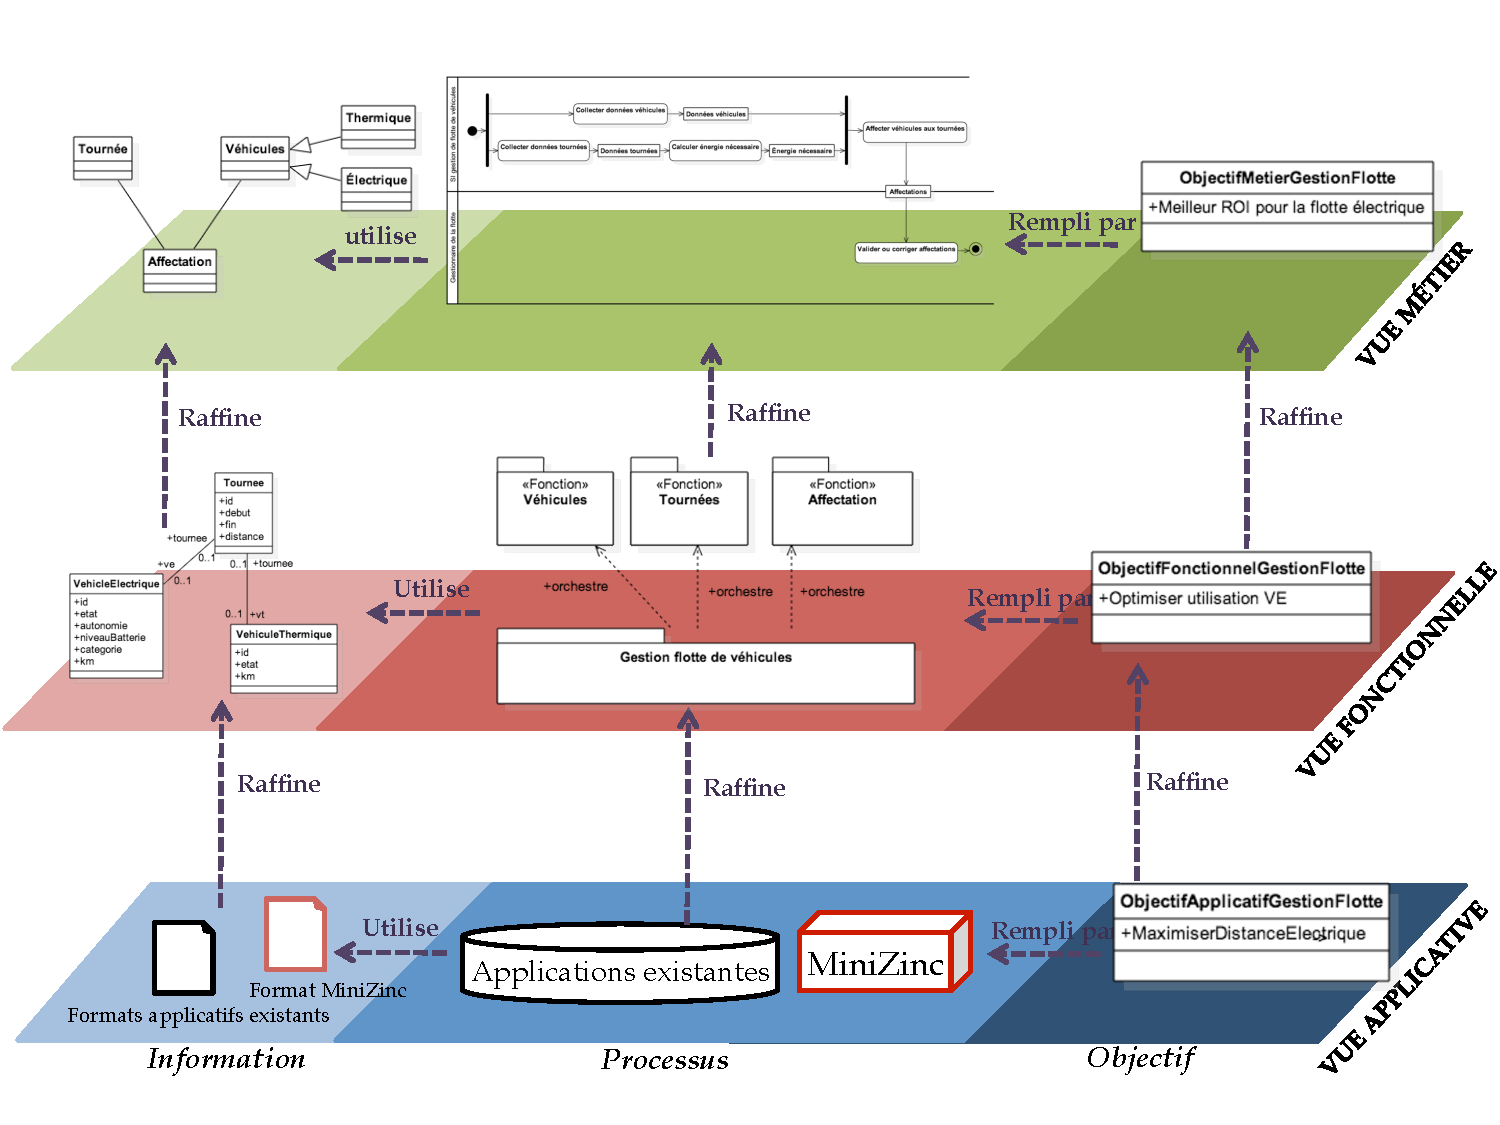
\includegraphics[angle=90, width=1\textwidth]{images/implementation/architecture_generale_usecase.pdf}
 \end{center}
 \caption{Approche conceptuelle pour l'analyse d'une architecture d'entreprise}
 \label{fig:architecture_generale_usecase}
\end{figure}


\subsubsection{Vue métier}
Nous utilisons fUML comme langage exécutable pour modéliser cette vue. Le processus métier consiste à collecter les données relatives aux véhicules (électriques et thermiques) ainsi qu'aux tournées à effectuer, de calculer l'énergie nécessaire à chaque tournée et l'affectation véhicule/tournée avant de faire valider cette dernière par le manager de flotte. Nous modélisons ce processus métier sous forme de diagramme d'activité fUML et le simulons en utilisant Papyrus. Selon notre cadre d'architecture, les modèles créés représentent donc l'aspect processus de la vue métier.

Pour l'aspect information, nous utilisons des diagrammes de classe UML pour représenter les concepts métier et leurs relations. Nous modélisons ainsi les concepts de Véhicule, Tournée et Affectation.
Gérer une flotte de véhicules peut avoir plusieurs objectifs métier. Dans notre cas, obtenir le meilleur retour sur investissement suite à l'intégration de véhicules électriques dans la flotte de véhicules. Nous modélisons l'objectif métier sous la forme d'une classe UML.

Le choix des langages de modélisation et de l'outil de simulation est motivé par les pratiques du domaine. En effet, la Commission Électrique Internationale a adopté Enterprise Architect comme outil pour maintenir et distribuer le CIM\footnote{Common Information Model}\cite{uslar2012standardization}, un modèle d'information commun pour le domaine électrique \footnote{www.sparxsystems.com.au/press/articles/iec.html}.
	

\subsubsection{Vue fonctionnelle}

Nous modélisons l'aspect information sous la forme d'une diagramme de classe fUML. Ce modèle raffine les concepts métier en spécifiant leurs types. Dans la vue fonctionnelle, le concept d'allocation prend la forme d'une association entre les véhicules et les tournées. L'objectif fonctionnel est modélisé sous la forme d'une classe UML. L'objectif fonctionnel spécifie qu'il faut optimiser l'utilisation des véhicules électriques pour atteindre l'objectif métier qui est d'avoir un meilleur retour sur investissement.

Pour l'aspect processus, nous commençons par identifier trois blocs fonctionnels : un bloc pour la gestion de la flotte de véhicules (électriques et thermiques), un bloc pour la gestion des tournées, un bloc pour la gestion de l'affectation (voir figure \ref{fig:architecture_generale_usecase}. Ces blocs contiennent les fonctions qui raffinent les tâches du processus métier. Comme expliqué plus tôt dans la démarche, le fait de les rassembler dans des blocs selon les concepts métier augmente la modularité et l'évoluvilité de l'architecture. De plus, nous consacrons un bloc à la gestion des processus fonctionnels. Ce bloc est responsable de l'orchestration des fonctions du processus fonctionnel. 

Les blocs fonctionnels offrent une vue plus détaillée des tâches métier. Il est possible de modéliser les différentes fonctions (calcul des tournées à partir de bon de travaux, calcul de l'énergie nécessaire à une tournée, etc.) à l'aide de diagrammes d'activité exécutables. Le choix du langage de modélisation dépend du cas d'application. Par exemple, nous modélisons l'affectation véhicule/tournée sous la forme de contraintes OCL~:~pour affecter un véhicule à une tournée, il faut que l'énergie nécessaire à celle-ci soit inférieure à l'autonomie de la batterie. Dans notre cas d'application, nous considérons qu'il n'est pas possible de recharge le véhicule pendant la tournée de l'agent.

Nous considérons un premier cas où il n'est pas possible de recharger la batterie au cours de la tournée. L'aspect \emph{information} de la vue fonctionnelle prend la forme de données fonctionnelles  modélisées par un diagramme de classes sur lequel s'appliquent les contraintes OCL (\ref{fig:architecture_generale_usecase}). OCL est adapté aux diagrammes de classes. De plus, OCL est un langage standardisé et exécutable pour l'expression de contraintes. Il est possible de modéliser les autres algorithmes de traitement (calcul des tournées à partir de bon de travaux, calcul de l'énergie nécessaire à une tournée, etc.) à l'aide de diagrammes d'activité exécutables.

En utilisant le langage OCL, nous modélisons la fonction d'affectation sous la forme de deux contraintes et d'une requête. La première contrainte OCL signifie que si un véhicule électrique est affecté à une tournée alors l'énergie dont il dispose permet d'assurer la totalité de la tournée.
La deuxième contrainte signifie que si aucun véhicule électrique n'est capable d'assurer une tournée donnée alors c'est un véhicule thermique qui lui est associé. Enfin, la requête calcule le nombre total de kilomètres électriques correspondant à la distance parcourue par les véhicules électrique après l'affectation. Cette requête permet d'évaluer l'utilisation  des véhicules électriques dans l'optique d'atteindre l'objectif fonctionnel.

\begin{queryl}[linewidth=15cm]
context Tournee
inv : 
self.ve.autonomie * self.ve.niveauBatterie > self.energieRequise

context Tournee
inv : self.ve <> undefined xor self.vt <> undefined

context Tournee :: elecKm() : int
body :  
(Tournee::allInstances() -> collect(t.ve <> undefined|t.distance)) 
-> sum()
\end{queryl}


\subsubsection{Vue applicative}

Pour les processus applicatifs, nous commençons par identifier 
les applications nécessaires à l'implantation des blocs fonctionnels. Dans notre cas, le patrimoine applicatif de l'entreprise dispose déjà d'applications pour la gestion de tournées (calcul de tournées optimisé à partir de bons de travaux) et la gestion de véhicules (administration, maintenance, etc.). Pour la fonction d'allocation, nous faisons le choix d'utiliser MiniZinc pour modéliser les contraintes au niveau applicatif \ref{fig:contraintesMiniZinc}. 

\begin{figure}[!htbp]
 \begin{center}
  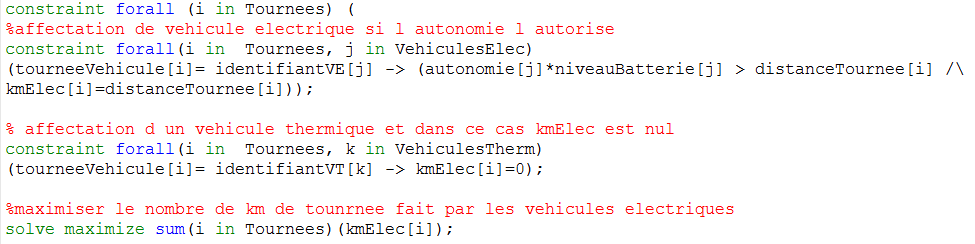
\includegraphics[width=1\textwidth]{images/implementation/module_minizinc.png}
 \end{center}
 \caption{Contraintes du module MiniZinc}
 \label{fig:contraintesMiniZinc}
\end{figure} 

MiniZinc est un langage de modélisation et de résolution de contraintes de niveau intermédiaire qui a pour vocation de devenir un langage de modélisation standard dans le domaine de la programmation par contraintes. L'aspect information contient les formats de données nécessaires aux différentes applications. La figure \ref{fig:formatMiniZinc} représente le fichier de données (le format .dzn) nécessaire à l'application MiniZinc pour calculer l'affectation. 

\begin{figure}[!htbp]
 \begin{center}
  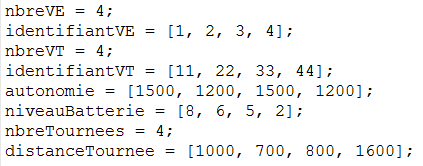
\includegraphics[width=0.5\textwidth]{images/implementation/format_minizinc.png}
 \end{center}
 \caption{Fichier de données pour le module MiniZinc}
 \label{fig:formatMiniZinc}
\end{figure} 

L'objectif applicatif est modélisé sous la forme d'une classe fUML. Un véhicule électrique devient rentable par rapport à un véhicule thermique à partir d'un certain nombre de kilomètre parcouru. C'est pourquoi l'objectif fonctionnel qui est d'optimiser l'usage de la flotte électrique se traduit par la maximisation du nombre de kilomètres électriques, c'est à dire affecter aussi souvent que possible un véhicule électrique aux tournées. Ainsi, le module MiniZinc prend en compte cet objectif en résolvant les contraintes tout en maximisant la distance électrique. 

\subsubsection{Vue intégration}

Nous modélisons la vue intégrative en spécifiant les liens de cohérence  intra-vue et et inter-vues. Les contraintes que ces liens doivent respecter sont spécifiés dans le métamodèle du cadre d'architecture présenté dans la démarche. La figure \ref{fig:integration_gestion_flotte} offre une vue partielle des modèles d'intégration. Nous y modélisons à titre illustratif les liens de cohérence intravue entre la fonction d'affection, ses inputs et output et son objectifs fonctionnel. Nous faisons de même pour le module d'optimisation Minizinc, ses inputs et outputs ainsi que l'objectif applicatif qu'il remplit. Le même principe est appliqué à tous les autres éléments de la vue métier, fonctionnelle et applicative. Nous mettons l'ensemble des modèles de la vue intégration en annexe de ce manuscrit. 

\begin{figure}[!htbp]
 \begin{center}
  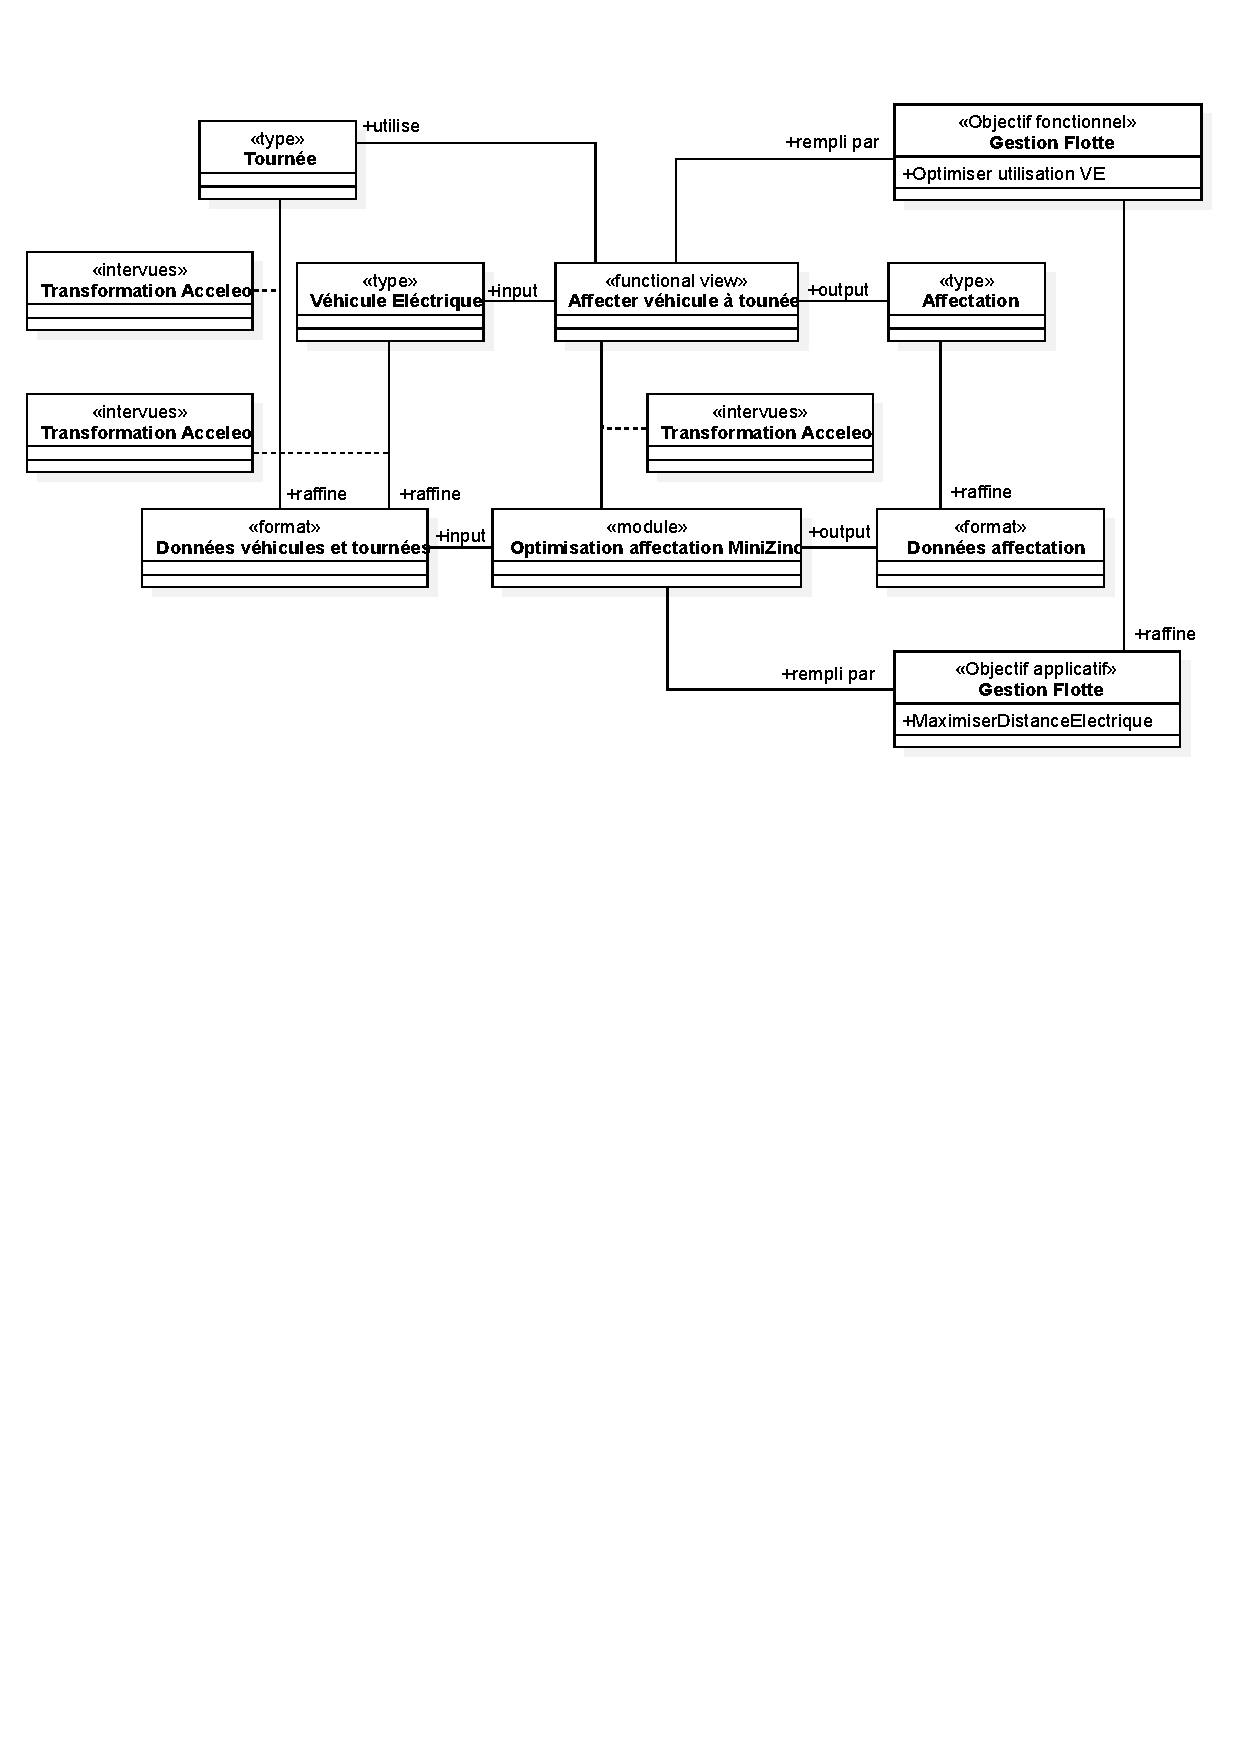
\includegraphics[trim= 0cm 16cm 0cm 0cm, width=1\textwidth]{images/implementation/integration_affection_gestion.pdf}
 \end{center}
 \caption{Une vue partielle des modèles d'intégration de la vue fonctionnelle et de la vue applicative}
 \label{fig:integration_gestion_flotte}
\end{figure}

Validate modèle -> pour tester l'intégrité du modèle
Détecter les problèmes d'interop' entre modules


For instance, an “input” link should check that the
information type is consistent with the function using it
and check that the information format fits the
application module involved. Besides, these constraints
ensure a good orchestration of tasks, functions and
modules. For example, it ensures that the output of a
given function is consistent with the input of the next
function. The links “input”, “output”, and “fulfilled by”
inherit from the class “Horizontal” of the metamodel of
our approach as illustrated in Figure 4.

